\documentclass[a4paper,ngerman,11pt,bibtotoc]{scrartcl}

\usepackage[utf8]{inputenc}

\usepackage[ngerman]{babel}

\usepackage{amsmath, amsthm, amssymb, stmaryrd, color, graphicx, mathtools, mathrsfs}
\usepackage{setspace}
\usepackage{bussproofs}
\usepackage{array}
\usepackage{booktabs}
\usepackage{comment}
\usepackage{textcomp}
\usepackage{stmaryrd}

\usepackage{tikz}
\usetikzlibrary{shapes,arrows}

\usepackage[protrusion=true,expansion=true]{microtype}

\usepackage{lmodern}
\usepackage{tabto}

\usepackage[backend=bibtex,style=alphabetic]{biblatex}
\usepackage[babel]{csquotes}
\bibliography{literatur}

\usepackage{titling}

\usepackage[all]{xy}

\usepackage[colorlinks=true, linkcolor=blue, urlcolor=blue, citecolor=blue]{hyperref}
\usepackage{cleveref}			% Referenzen mit Name

\usepackage{icomma}				% Korrektes Typesetting von Kommazahlen

\usepackage[font={small,it}]{caption} % Kleinere Captions


\usepackage{algorithm}
\usepackage{algpseudocode}
\algrenewcommand{\algorithmiccomment}[1]{\hskip3em$\slash\slash$ #1}
\newcommand{\LineFor}[2]{\State\algorithmicfor\ {#1}\ \algorithmicdo\ {#2} \algorithmicend\ \algorithmicfor}

\usepackage{listings}			% Anzeige von Sourcecode

\setlength\parskip{\medskipamount}
\setlength\parindent{0pt}

\theoremstyle{definition}
\newtheorem{defn}{Definition}[section]
\newtheorem{axiom}[defn]{Axiom}
\newtheorem{bsp}[defn]{Beispiel}

\theoremstyle{plain}

\newtheorem{prop}[defn]{Proposition}
\newtheorem{motto}[defn]{Motto}
\newtheorem{ueberlegung}[defn]{Überlegung}
\newtheorem{lemma}[defn]{Lemma}
\newtheorem{kor}[defn]{Korollar}
\newtheorem{hilfsaussage}[defn]{Hilfsaussage}
\newtheorem{satz}[defn]{Satz}

\theoremstyle{remark}
\newtheorem{erin}[defn]{Erinnerung}
\newtheorem{bem}[defn]{Bemerkung}
\newtheorem{beob}[defn]{Beobachtung}
\newtheorem{aufg}[defn]{Aufgabe}

\clubpenalty=10000
\widowpenalty=10000
\displaywidowpenalty=10000

\newcommand{\IZ}{\mathbb{Z}}
\newcommand{\IQ}{\mathbb{Q}}
\newcommand{\IR}{\mathbb{R}}
\newcommand{\IC}{\mathbb{C}}
\newcommand{\IN}{\mathbb{N}}
\newcommand{\Ic}{\mathcal{I}}
\newcommand{\Jc}{\mathcal{J}}
\newcommand{\Hc}{\mathcal{H}}
\newcommand{\Tc}{\mathcal{T}}
\newcommand{\Sc}{\mathcal{S}}
\newcommand{\Oc}{\mathcal{O}}

\newcommand{\ceil}[1]{\left\lceil#1\right\rceil}

% Nur für dieses Dokument %%%%%%%%%%%%%%%%%%%%%%%%%%%%%%%%%%%%%%

\newcommand{\ClientSet}{\mathscr{C}}
\newcommand{\FacilitySet}{\mathscr{F}}
\newcommand{\allTours}{\mathscr{T}}

\newcommand{\OPT}{OPT}
\newcommand{\CLR}{CLR}
\newcommand{\CLRHFC}{CLRhFC}
\newcommand{\MST}{MST}
\newcommand{\UFL}{UFL}

% C++ from http://tex.stackexchange.com/a/4304
\def\Cpp{{C\nolinebreak[4]\hspace{-.05em}\raisebox{.4ex}{\tiny\bf ++}}}

% Switch between equationsnumbers on the left and on the right (from http://tex.stackexchange.com/a/193538 )
\makeatletter
\newcommand{\leqnomode}{\tagsleft@true}
\newcommand{\reqnomode}{\tagsleft@false}
\makeatother

\renewcommand*\theenumi{\alph{enumi}}
\renewcommand{\labelenumi}{(\theenumi)}

% Set language and other options for Code snippets
\lstset{language=C++}
\lstset{tabsize=4}
\lstset{basicstyle=\small\ttfamily}
\lstset{frame=Tb, captionpos=b}
\lstset{xleftmargin=1em, xrightmargin=1em, aboveskip=2\medskipamount}
% Umlaute in Code:
\lstset{literate=%
	{Ö}{{\"O}}1
	{Ä}{{\"A}}1
	{Ü}{{\"U}}1
	{ü}{{\"u}}1
	{ä}{{\"a}}1
	{ö}{{\"o}}1
}
\definecolor{purplekeywords}{rgb}{0.5,0,0.33}
\definecolor{greencomments}{rgb}{0,0.5,0}
\definecolor{bluestrings}{rgb}{0,0,1}
\definecolor{types}{rgb}{0.17,0.57,0.68}
\lstset{
	commentstyle=\color{greencomments},
	morekeywords={},
	keywordstyle=\color{purplekeywords}\textbf,
	stringstyle=\color{bluestrings},
}

\setcounter{tocdepth}{3}


\usepackage{todonotes}
\usepackage{tabu}


% DOCUMENT %%%%%%%%%%%%%%%%%%%%%%%%%%%%%%%%%%%%%%%%%%%%%%%%%%%%%

\begin{document}
\author{Lukas Graf}
\date{Letzte Aktualisierung: \today}

\selectlanguage{ngerman}
\thispagestyle{empty}


\begin{titlepage}\center
	\textsc{\LARGE Universität Augsburg}\\[1cm]
	
	\textsc{\Large Institut für Mathematik}\\[1.5cm]
	
	% Title
	{\Large Ausarbeitung \\[1cm]}
	zum mathematischen Softwareprojekt\\[1cm]
	{\huge Capacitated Location Routing \\ with Hard Facility Capacities}

	\begin{center}
		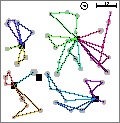
\includegraphics[width=.6\textwidth]{bilder/title.pdf}
	\end{center}		
	
	\vfill
	
	% Author and supervisor
	\begin{minipage}{0.4\textwidth}
		\begin{flushleft} \large
			\emph{von:}\\
			Lukas \textsc{Graf}
		\end{flushleft}
	\end{minipage}
	\begin{minipage}{0.4\textwidth}
		\begin{flushright} \large
			\emph{Betreut von:} \\
			Prof. Dr. Tobias \textsc{Harks}
		\end{flushright}
	\end{minipage}
	
\end{titlepage}

% CONTENT %%%%%%%%%%%%%%%%%%%%%%%%%%%%%%%%%%%%%%%%%%%


\tableofcontents

\newpage
	
\section*{Einleitung}

Gegeben eine Menge von Kunden mit unterschiedlich großen Bedarfen nach einem einheitlichen Gut, eine Menge möglicher Fabrikstandorte mit jeweils verschiedenen Eröffnungskosten, eine unbegrenzte Anzahl von Lieferfahrzeugen mit einheitlicher Kapazität sowie eine metrische Abstandsfunktion auf der Gesamtmenge. Welche Standorte sollte man eröffnen und wie sollte man die Fahrzeuge einsetzen um die Bedarfe aller Kunden zu erfüllen und dabei die Summe der Kosten für Fabrikeröffnungen und gefahrene Strecken zu minimieren?

Diese Fragestellung wird im \emph{Capacitated Location Routing}-Problem (\CLR) formalisiert, einem NP-schweren Optimierungsproblem.

Da es also vermutlich keinen polynomiellen exakten Algorithmus hierfür gibt, interessiert man sich dafür polynomielle Approximationsalgorithmen hierfür zu finden. Einen solchen $4,38$-approximativen Algorithmus beschrieben und implementierten Harks, König und Matuschke in \cite{AAfCLR}. 

Aufbauend auf diesem existierenden Programm habe ich im Rahmen des hier beschriebenen Softwareprojekts zwei Ergänzungen zu diesem Algorithmus bzw. dessen Implementierung vorgenommen: Es wurde die Möglichkeit hinzugefügt das Ergebnis sowie verschiedene Zwischenschritte des Algorithmus graphisch auszugeben. Der Algorithmus selbst wurde um zwei Varianten ergänzt, die nun zusätzlich mit Kapazitätsbeschränkungen der Fabriken umgehen können, und weiterhin zulässige Lösungen finden (allerdings ohne garantierte Approximationsgüte).

In der folgenden Ausarbeitung wird zunächst kurz der bestehende Algorithmus für \CLR{} skizziert und dann die Implementierung der beiden neuen Bestandteile beschrieben. Schließlich wird der erweiterte Algorithmus auf einigen Instanzen getestet.


\newpage

\section{Capacitated Location Routing (\CLR)}

	\subsection{Problemdefinition}

Eine Instanz des \textbf{Capacitated Location Routing Problems (\CLR)} ist gegeben durch
\begin{itemize}
	\item einen ungerichteten, zusammenhängenden Graphen $G =(V,E)$,
	\item eine Partition der Knoten in Kunden $\ClientSet$ und Fabrikstandorte $\FacilitySet$,
	\item eine metrischen Kostenfunktion auf den Kanten $c: E \to \IR_{\geq 0}$,
	\item Eröffnungskosten für die Fabriken $\phi: \FacilitySet \to \IR_{\geq 0}$,
	\item Bedarfe der Kunden $d: \ClientSet \to \IR_{\geq 0}$
	\item und eine einheitliche Kapazität $u > 0$ für die Fahrzeuge.		
\end{itemize}
Zulässige Lösungen bestehen aus
\begin{itemize}
	\item einer Teilmenge $F \subseteq \FacilitySet$ von eröffneten Fabriken
	\item und einer Menge von Touren $\Tc = \{T_1, \dots, T_k\}$,
\end{itemize}
sodass gilt:
\begin{itemize}
	\item Zu jeder Tour gibt es eine geöffnete Fabrik $f \in F$, an der diese startet und endet.
	\item Alle Touren zusammen erfüllen alle Bedarfe der Kunden.
	\item Keine der Touren übersteigt die Kapazität $u$.
\end{itemize}
Das Optimierungsziel ist es die Gesamtkosten für das Eröffnen der Fabriken und die gefahrenen Touren zu minimieren, also die Minimierung der Kostenfunktion
\footnote{Wir verwenden hier, dass eine $\IR$-wertige Funktion $c: M \to \IR$ auf einer beliebigen Menge $M$ eine Funktion $\tilde{c}: \mathcal{P}(M) \to \IR: M \supseteq N \mapsto \sum_{x \in N} c(x)$ auf der Potenzmenge $\mathcal{P}(M)$ induziert. Zur Vereinfachung der Notation bezeichnen wir diese Funktion dann ebenfalls mit $c$. Unter nochmaliger Anwendung dieser Konvention ließe sich die obige Kostenfunktion daher noch kürzer als $c(\Tc) + \phi(F)$ schreiben.}
	\[\sum_{T\in\Tc} c(T) + \sum_{f\in F}\phi(f) \]
	
\begin{beob}
	$\CLR{}$ ist NP-schwer, denn es beinhaltet beispielsweise metrisches TSP (betrachte Instanzen mit $|\FacilitySet| = 1$, $d \equiv 1$ und $u = |\ClientSet|$).
\end{beob}

\begin{bem}
	Gilt $d \equiv 1$ und $u = 1$, so erhält man eine Instanz des (metrischen) \emph{Uncapacitated Facility Location Problems} (\UFL). Statt Touren von den geöffneten Fabriken zu den Kunden zu finden, genügt es hier offensichtlich eine Zuordnung von Kunden zu Fabriken zu bestimmen. Für dieses Problem sind eine ganze Reihe von Approximationsalgorithmen bekannt (vergleiche z.B. \cite{AAfFLP}), unter anderem erweist sich ein einfacher Greedy-Ansatz bereits als $1,861$-approximativ (siehe \cite{GreedyApprox}).
\end{bem}


	\subsection{Ein Approximationsalgorithmus für \CLR}

Der in \cite{AAfCLR} beschriebene $4,38$-approximative\footnote{Die diesem Softwareprojekt zugrunde liegende Implementierung weist allerdings nur eine Approximationsgarantie von $5,722$ auf, da zur approximativen Lösung der \UFL-Instanz ein leichter zu implementierender Greedy-Algorithmus verwendet wurde, anstatt des im Beweis zitierten Algorithmus mit besserer Approximationsgarantie.} Algorithmus für \CLR{} basiert im Wesentlichen auf den folgenden Schritten (schematisch dargestellt in \cref{fig:CLRAlg}):
\begin{description}
	\item[\UFL-Phase:] Erstelle eine \UFL-Instanz mit den gleichen Fabriken und Kunden, aber mit um $2/u$ skalierten Kosten. Löse diese Instanz approximativ und eröffne alle hier geöffneten Fabriken auch in der \CLR-Instanz. Es zeigt sich, dass die Kosten einer optimalen Lösung der \UFL-Instanz eine untere Schranke für die optimale Lösung der \CLR-Instanz bilden.
	\item[\MST-Phase:] Ergänze den Graphen der \CLR-Instanz um einen zusätzlichen Knoten $r$ mit kostenlosen Kanten zu allen Fabriken. Erhöhe ferner die Kosten aller Kanten zwischen Fabriken und Kunden um die halben Eröffnungskosten der jeweiligen Fabrik. Dann finde einen minimalen Spannbaum $B$ in diesem Graphen und öffne in der \CLR-Instanz zusätzlich alle Fabriken, die in $B$ wenigstens einen Kunden als Nachbarn haben. Die Kosten eines solchen Spannbaumes sind erneut eine untere Schranke für die Kosten einer optimalen Lösung der \CLR-Instanz.
	\item[Large Demand-Phase:] Alle Kunden mit Bedarf von mindestens $u$ werden durch $\ceil{d/u}$ Touren mit der jeweils nächsten Fabrik verbunden. Die hierfür anfallenden Anbindungskosten sind höchstens zweimal die entsprechenden Kosten aus der \UFL-Phase.
	\item[Merge-Phase] Betrachte $B$ aus der \MST-Phase als Baum mit Wurzel $r$. Solange dies möglich ist, finde darin einen Teilbaum (mit Wurzel $v$), der einen Gesamtbedarf von mehr als $u$ hat, aber dessen nächstkleinere Teilbäume (beginnend bei den Kindern von $v$) einen Bedarf von höchstens $u$ haben. Ein solcher Baum wird als \emph{Relieve-Tree} bezeichnet.
	 
	Fasse dessen kleineren Teilbäume und den \glqq Baum\grqq{} $\{v\}$ so zusammen, dass jede Menge einen Bedarf zwischen $\frac{u}{2}$ und $u$ hat (die letzte ggfls. weniger). Wandle jede der großen Mengen in eine Tour um (durch Verdoppeln der Kanten im entsprechenden Teilbaum und nachfolgendes Abkürzen bei doppelt besuchten Kunden) und verbinde sie mit der nächstliegenden offenen Fabrik. Die Verbindungskosten hierfür sind beschränkt durch das Doppelte der Kosten im Spannbaum $B$ und den entsprechenden Verbindungskosten aus der \UFL-Phase. Die Kunden aus der kleinen Menge bleiben vorerst unversorgt und werden beim nächsten Relieve-Tree neu berücksichtigt.
	
	Ist der verbleibende Gesamtbedarf unter einer Fabrik schließlich kleiner oder gleich $u$, so werden alle im entsprechenden Teilbaum verbliebenen Kunden zu einer Tour (\emph{Remaining-Tour}) zusammengefasst und mit der nächstliegenden offenen Fabrik verbunden. Die Verbindungskosten hierfür sind erneut durch das Doppelte der entsprechenden Kosten aus dem Spannbaum begrenzt.
\end{description}

\begin{figure}[H]
	\begin{tiny}
		
\tikzstyle{Absch} = [rectangle, draw, 
    text centered]
\tikzstyle{keinBeweis} = [rectangle, fill=gray!25, 
    text centered]    

\tikzstyle{BewTeil} = []


\tikzstyle{Box} = [rectangle, draw, text centered, rounded corners]
\tikzstyle{Alg} = [rectangle, draw, fill=gray!50, text centered]
\tikzstyle{Text} = [text centered]
\tikzstyle{Image} = []

\tikzstyle{arrow} = [draw, -latex']
\tikzstyle{line} = [draw]


\begin{tikzpicture}[node distance = 5em, auto]

% EINGABE:
\node [Box, text width=20em] (input) {\textbf{Input:} \\ CLR-Instanz $((\ClientSet\cup\FacilitySet,E),c,\phi,d,u)$};
\node [below of=input] (under-input) {};
\node [Image, above of=input, node distance=6em] (input-img) {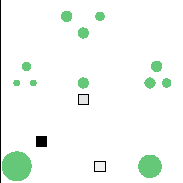
\includegraphics[width=8em]{bilder/instance.pdf}};

% ULF-Instanz:
\node [Box, left of=under-input, text width=14em, node distance=8em] (ULF) 
	{\textbf{ULF-Instanz:} \\ $((\ClientSet\cup\FacilitySet,E),\tilde{c},\phi,d)$ \\
	wobei $\tilde{c}:E \to \IR_{\geq 0}: e \mapsto \frac{2}{u}c(e)$};
\node [Text, left of=ULF, text width=12em, node distance=15em] (ULF-lower-bound) {$\leadsto$ Untere Schranke: $\OPT(\CLR) \geq \OPT(\ULF)$};
\node [Alg, below of=ULF, text width=14em] (ULF-solving) {löse approximativ (mit Greedy)};
\node [Image, left of=ULF-solving, node distance=15em] (ULF-img) {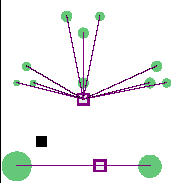
\includegraphics[width=5em]{bilder/ULF.pdf}};

% MST-Instanz:
\node [Box, right of=under-input, text width=14em, node distance=8em] (MST)
	{\textbf{MST-Instanz:} \\ $((\ClientSet\cup\FacilitySet\cup\{r\},E^\prime),c^\prime)$ \\
	$E^\prime := E \cup \{\{r,f\}\mid f\in\FacilitySet\}$ \\
	$c^\prime(f,v) := c(f,v) + \frac{1}{2}\phi(f),$ \\
	$c^\prime(r,f) := 0, c^\prime(v,w):=c(c,w)$};
\node [Text, right of=MST, text width=12em, node distance=15em] (MST-lower-bound) {$\leadsto$ Untere Schranke: $\OPT(\CLR) \geq \OPT(\MST)$};
\node [Alg, below of=MST, text width=14em] (MST-solving) {löse exakt (mit ???)};
\node [Image, right of=MST-solving, node distance=15em] (MST-img) {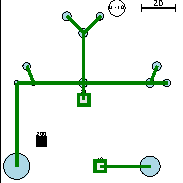
\includegraphics[width=5em]{bilder/MST.pdf}};

% MERGE-Phase:
\node [Text, below of=under-input, node distance=8em] (merge) {\textbf{Merge-Phase:}};

\node [Alg, below of=merge, node distance=1.5em, text width=30em] (m-facilities) {
		\begin{minipage}{30em}\begin{algorithmic}
		\State Eröffne in $\ULF$ oder $\MST$ verwendete Fabriken
		\end{algorithmic}\end{minipage}
	};
\node [Text, left of=m-facilities, node distance=25em, text width=15em] () 
	{beschränkt durch die entsprechenden Eröffnungskosten in $\ULF$ und $\MST$};

% Große Klienten
\node [Alg, below of=m-facilities, node distance=4em] (m-big-clients) {
		\begin{minipage}{30em}\begin{algorithmic}
		\For{Klienten $v$ mit $d(v)\geq u$}
			\State Verbinde $v$ durch $\frac{d(v)}{u}$ Touren mit nächster offener Fabrik
		\EndFor
		\end{algorithmic}\end{minipage}
	};
\node [Image, right of=m-big-clients, node distance=25em] () {
	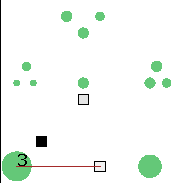
\includegraphics[width=5em]{bilder/largeDemand1.pdf}
	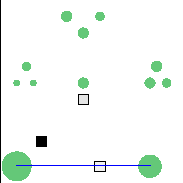
\includegraphics[width=5em]{bilder/largeDemand2.pdf}
};
\node [Text, left of=m-big-clients, node distance=25em, text width=15em] () 
	{beschränkt durch $2\times$ den entsprechenden Verbindungskosten in $\ULF$};

% Kleine Klienten
\node [Alg, below of=m-big-clients, node distance=4em] (m-small-clients) {
		\begin{minipage}{30em}\begin{algorithmic}\algtext*{EndFor}
		\For{Durch $\MST$ eröffnete Fabrik $f$ tue}
		\State Definitionen...
		\EndFor
		\end{algorithmic}\end{minipage}
	};

% Relieve-Schritte
\node [Alg, below of=m-small-clients, node distance=5em] (m-relieve) {
		\begin{minipage}{30em}\begin{algorithmic}\algtext*{For}\algtext*{EndFor}
			\For
			\While{$D_f > 0$}
			\State Finde $v \in S_f$ mit $D_v > u$ und f.a. Kinder $w$ von $v$: $D_w \leq u$
			\State Zerlege $S_v$ in Teilbäume ...
			\EndWhile
			\EndFor
			\end{algorithmic}\end{minipage}
	};
\node [Image, right of=m-relieve, node distance=25em] () {
		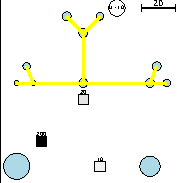
\includegraphics[width=5em]{bilder/relieveTour1.pdf}
		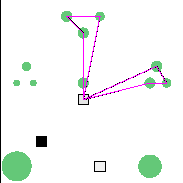
\includegraphics[width=5em]{bilder/relieveTour2.pdf}
		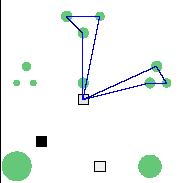
\includegraphics[width=5em]{bilder/relieveTour3.pdf}
	};
\node [Text, left of=m-relieve, node distance=25em, text width=15em] () 
	{Jede Tour ist beschränkt durch $2\times$ die Kantenkosten im $\MST$ und $2\times$ den Verbindungskosten aller Knoten der Tour in $\ULF$};

% Rest
\node [Alg, below of=m-relieve, node distance=5em] (m-remaining) {
		\begin{minipage}{30em}\begin{algorithmic}\algtext*{For}
		\For
		\State Mache Rest
		\EndFor
		\end{algorithmic}\end{minipage}
	};
\node [Image, right of=m-remaining, node distance=25em] () {
	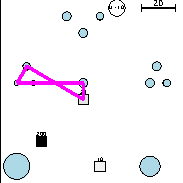
\includegraphics[width=5em]{bilder/remainingTour1.pdf}
	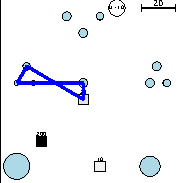
\includegraphics[width=5em]{bilder/remainingTour2.pdf}
};
\node [Text, left of=m-remaining, node distance=25em, text width=15em] () 
	{beschränkt durch $2\times$ den Verbindungskosten in $\MST$};


% AUSGABE:
\node [Box, below of=m-remaining, node distance=3em] (output) {\textbf{Output}};
\node [Image, below of=output] (outpu-img) {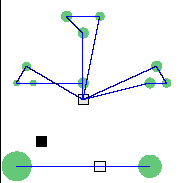
\includegraphics[width=8em]{bilder/output.pdf}};


% PATHS:

\path [arrow] (input.south) -- (ULF.north);    
\path [arrow] (input.south) -- (MST.north); 

\path [arrow] (ULF) -- (ULF-solving.north);
\path [arrow] (MST) -- (MST-solving.north);
\path [arrow] (ULF-solving.south) -- (merge.north);
\path [arrow] (MST-solving.south) -- (merge.north);

\path [line] (m-facilities) -- (m-big-clients);
\path [line] (m-big-clients) -- (m-small-clients);
\path [line] (m-small-clients) -- (m-relieve);
\path [line] (m-relieve) -- (m-remaining);

\path [arrow] (m-remaining.south) -- (output.north);

\end{tikzpicture}

	\end{tiny}
	\caption{Schematische Darstellung des Algorithmus für CLR}\label{fig:CLRAlg}
\end{figure}

\subsection{Visualisierung des Algorithmus}

Im ersten Teil des Softwareprojektes ging es darum den Ablauf sowie das Ergebnis des oben beschriebenen Algorithmus zu visualisieren. Dazu habe ich die existierende Implementierung des Algorithmus um eine Klasse \lstinline|CLR_Drawing| erweitert. Diese bietet die Möglichkeit das Ergebnis sowie verschiedene Zwischenstadien des Algorithmus graphisch abzubilden. 

Die Ausgabe besteht aus SVG-Dateien, die mit Hilfe der \Cpp-Bibliothek simple-svg (\cite{simple-svg}) erstellt werden. Diese können dann beispielsweise von Hand übereinander gelegt werden, um ein bestimmtes Zwischenstadium des Algorithmus darzustellen, oder zu einer Animation zusammengesetzt werden, um den gesamten Ablauf des Algorithmus abzubilden.

Ein Beispiel für ersteres sind die Bilder in dieser Arbeit, ein Beispiel für Letzteres kann man auf \url{http://graffl.github.io/misc/drawings/drawings-steps.html} sehen.

\begin{figure}[H]\centering\setlength{\fboxsep}{0pt}
	\fbox{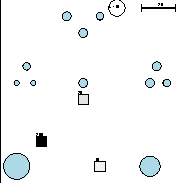
\includegraphics[width=.19\textwidth]{bilder/demo_instance.pdf}}
	\fbox{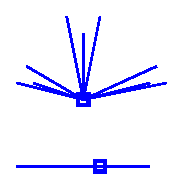
\includegraphics[width=.19\textwidth]{bilder/demo_UFL.pdf}}
	\fbox{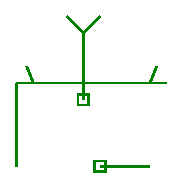
\includegraphics[width=.19\textwidth]{bilder/demo_Tree.pdf}}
	\fbox{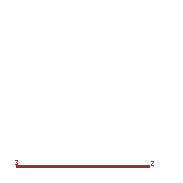
\includegraphics[width=.19\textwidth]{bilder/demo_LargeDemand.pdf}}
	\fbox{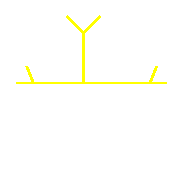
\includegraphics[width=.19\textwidth]{bilder/demo_relieveTree.pdf}}
	
	\fbox{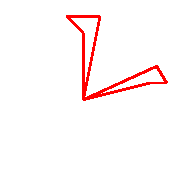
\includegraphics[width=.19\textwidth]{bilder/demo_relieveTour.pdf}}
	\fbox{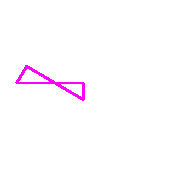
\includegraphics[width=.19\textwidth]{bilder/demo_remainingTour.pdf}}
	\fbox{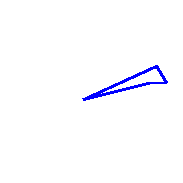
\includegraphics[width=.19\textwidth]{bilder/demo_singleTour.pdf}}
	\fbox{
\includegraphics[width=.19\textwidth]{bilder/demo_allTours.pdf}}
	
	\caption{Ausgaben der Klasse \lstinline|CLR_Drawing|: Die Instanz selbst, die Lösung der UFL-Instanz, die Lösung der MST-Instanz, Touren aus der Large-Demand-Phase, ein Relieve-Tree, daraus entstandene Relieve-Touren, eine Remaining-Tour, eine einzelne Tour, alle Touren}
\end{figure}

Die Klasse \lstinline|CLR-Drawing| ist als Singelton implementiert, wodurch zum einen sicher gestellt ist, dass immer nur eine Instanz dieser Klasse existiert, und zum anderen jede Funktion auf die Instanz zugreifen kann, ohne das diese jeweils explizit übergeben werden muss. 

Zu Beginn des Algorithmus muss die Klasse mit allen Daten der Instanz initialisiert werden (etwa indem die entsprechende Datei übergeben wird). Ab dann kann jederzeit im Laufe des Algorithmus eine der Zeichnen-Funktionen der Klasse aufgerufen werden, um eine SVG-Datei zu erzeugen, die den entsprechenden Zwischenschritt darstellt (bspw. die Lösung der \UFL-Instanz, das Ergebnis der Large Demand-Phase oder eine einzelne Tour).

Die Namen der hierbei erzeugten Dateien sowie die Farben der verschiedenen Elemente sind momentan innerhalb der Klasse fest einprogrammiert. Lediglich bei der Funktion \lstinline|draw_tours()|, die ein Bild aller gefundenen Touren erzeugt, ist es bereits möglich zu entscheiden, ob alle Touren in einer einheitlichen Farbe (lila) dargestellt werden oder jede Tour eine andere Farbe bekommt, damit man die einzelnen Touren leichter unterscheiden kann.

Das Bild der Instanz stellt Kunden als Kreise und Fabriken als Quadrate dar. Die Fläche der geometrischen Formen ist dabei proportional zum jeweiligen Bedarf des Kunden bzw. der Kapazität der Fabrik (letzteres nur für echte \CLRHFC-Instanzen). Bei Fabriken entspricht zusätzlich die Schattierung des Quadrates der Höhe der Eröffnungskosten (je teurer, desto dunkler). Diese werden außerdem als kleine Zahl über der jeweiligen Fabrik angegeben. Schließlich wird noch am oberen rechten Rand des Bildes ein Maßstab für die Entfernungen und ein die Fahrzeugkapazität repräsentierender Kreis dargestellt.

\begin{lstlisting}[caption=Die Klasse \lstinline|CLR_Drawing| (gekürzt)]
class CLR_Drawing {
private:
CLR_Drawing() {...};

public:
static CLR_Drawing* get_instance() {
	static CLR_Drawing instance;
	return &instance;
}

// Verschiedene Möglichkeiten der Initialisierung:
bool init(vector<vector<double> > c_pos, vector<vector<double> > 
d_pos, vector<double> dems, vector<double> oCosts, double u);
bool init(const char* fileName);
bool init(const char* fileName, bool fac_cap_relevant);
bool init(); // Wenn keine Zeichnungen erstellt werden sollen

// Zeichnet die Instanz selbst (Kunden, Fabrikstandorte, Legende)
void draw_instance();
// Zeichnet Lösung der UFL-Instanz:
void draw_UFL_solution(vector<bool> facOpen, vector<int> facForClient);
// Zeichnet den in der MST-Phase gefundenen Spannbaum:
void draw_tree(Tree tree);
// Zeichnet eine einzelne Tour in die übergebene SVG-Datei:
void draw_tour(list<int> tour, svg::Color color, svg::Document* doc);
void draw_tour(list<int> tour, svg::Color color, string filename);
// Zeichnet das Ergebnis der Large Demand-Phase:
void draw_largeDemandPhase(list<vector<int> > tours_for_drawing);
// Zeichnet einen Relieve-Baum:
void draw_relieve_tree(Tree tree, int root, vector<bool> served);
// Zeichnet eine Relieve-Tour:
void draw_relieve_tours(list<list<int> > tours);
// Zeichnet eine Remaining-Tour:
void draw_remaining_tour(list<int> tour);
// Zeichnet alle bisher gefundenen Touren:
void draw_current_tours(list<list<int> > tours);
// Zeichnet alle übergebenen Touren
// (monochrome=false -> jede Tour in eigener Farbe):
void draw_tours(list<list<int> > tours, bool monochrome = true);
};
\end{lstlisting}

Für sich genommen kann die Klasse \lstinline|CLR_Drawing| außerdem auch dazu verwendet werden, anderweitig gefundene Touren für bestimmte Instanzen zu zeichnen. Dies ist zum Beispiel hilfreich, wenn man eine mittels eines MIP-Solvers gefundene optimale Lösung zeichnen lassen möchte. Dazu habe ich ein eigenes Programm \lstinline|DrawTours| angelegt, dem zwei Dateien (eine die Instanz beschreibende und eine für die Touren) übergeben werden können, und welches daraus entsprechende Bilder generiert.


\section{\CLR{} with Hard Facility Capacities (\CLRHFC)}

Eine Verallgemeinerung von \CLR{} erhält man, indem man die Kapazitäten der Fabriken beschränkt. In diesem Kapitel geht es darum, wie der Approximationsalgorithmus für \CLR{} so angepasst werden kann, dass er auch für das neue Problem zulässige Lösungen findet.

	\subsection{Problemdefinition}\label{sec:CLRHFC-Def}

Eine Instanz von \textbf{Capacitated Location Routing with Hard Facility Capacities (\CLRHFC)} ist gegeben durch:
\begin{itemize}
	\item eine Instanz $(G=(\ClientSet\cup\FacilitySet,E), c,\phi,d,u)$ von \CLR
	\item und zusätzlich Kapazitäten der Fabriken $l: \FacilitySet \to \IR_{\geq 0}$.
\end{itemize}
Zulässige Lösungen sind Lösungen der zugrunde liegenden \CLR-Instanz, die zudem die Kapazitätsschranken der Fabriken einhalten.

Das Optimierungsziel ist weiterhin die Minimierung der unveränderten Kostenfunktion der \CLR-Instanz.

\begin{bem}
Im Gegensatz zu den hier verwendeten \emph{harten Fabrikkapazitäten} gibt es auch Varianten von \CLR{} mit \emph{weichen Fabrikkapazitäten}. Dies bedeutet, dass die Fabriken zwar beschränkte Kapazität haben, jedoch mehrfach eröffnet werden dürfen, wodurch die Kapazität (aber natürlich auch die Eröffnungskosten) entsprechend vervielfacht werden (siehe z.B. \cite{SoftCap1}).  
\end{bem}

\CLRHFC{} kann auch als Mixed Integer Program (MIP) beschrieben werden. Dabei gibt es
\begin{itemize}
	\item für jede Fabrik eine Variable $o_f$, welche bestimmt, ob die entsprechende Fabrik geöffnet ($1$) ist oder nicht ($0$),
	\item sowie für jede mögliche Tour $T$ eine Variabel $y_T$, welche bestimmt, wie oft die entsprechende Tour genutzt wird,
	\item und für jeden auf $T$ liegenden Kunden $v$ eine Variable $x_{vT}$, welche besagt, wie viele Einheiten durch Tour $T$ insgesamt an den Kunden $v$ geliefert werden.
\end{itemize}

Das MIP sieht dann wie folgt aus:

\setlength{\fboxsep}{5pt}
\fbox{
\begin{minipage}[H]{.43\textwidth}\small\leqnomode
\begin{center}
	minimiere
	\begin{align*}\sum_{f \in \FacilitySet} o_f \phi(f) + \sum_{T \in \allTours} y_T c(T)\end{align*}
	unter den Nebenbedingungen:
	\begin{align}	\sum_{v \in T\cap\ClientSet} x_{vT} \leq u y_T 						&,\quad T \in \allTours 						\\
	\sum_{T \in \allTours_f} \sum_{v \in T\cap\ClientSet} x_{vT} \leq o_f l(f)			&,\quad f \in \FacilitySet						\\
	\sum_{T \in \allTours: v \in T} x_{vT} \geq d(v)									&,\quad v \in \ClientSet					
	\end{align}
	wobei
	\begin{align*}o_f \in \{0,1\},\quad y_T \in \IN_0, \quad x_{vT} \geq 0\end{align*}
\end{center}
\end{minipage}
\begin{minipage}[H]{.53\textwidth}\small
	Die (zu minimierenden) Gesamtkosten ergeben sich als Summe der Eröffnungskosten $\phi(f)$ und der Tourkosten $c(T)$.
	
	
	\begin{enumerate}\renewcommand{\theenumi}{\arabic{enumi}}
		\item Die Fahrzeugkapazität $u$ wird eingehalten. D.h. wird eine Tour $y_T$-mal genutzt, so können durch sie höchstens $u y_T$ Einheiten an die auf ihr liegenden Kunden geliefert werden.
		\item Die Fabrikkapazitäten $l$ werden eingehalten. Alle bei eine Fabrik $f$ beginnenden Touren ($\allTours_f$) können zusammen höchstens so viele Einheiten ausliefern, wie die Fabrikkapazität $l(f)$ zulässt (und $f$ muss geöffnet sein).
		\item Die Bedarfe der Kunden $d$ werden erfüllt. Dies ist der Fall, wenn alle Touren, auf denen ein Kunde $v$ liegt, zusammen mindestens so viel an ihn liefern, wie sein Bedarf $d(v)$ ist.
	\end{enumerate}
\end{minipage}
}\vspace{1em}

\begin{beob}
	Die Menge aller denkbaren Touren $\allTours$ wächst exponentiell in der Zahl der Kunden der \CLRHFC-Instanz (genauer $|\allTours| = m \sum_{k=1}^{n} {n \choose k}k!$, wobei $m := |\FacilitySet|, n := |\ClientSet|$). Dementsprechend schnell steigt auch die Zahl der Variablen und der Nebenbedingungen an, sodass das Problem nur für sehr kleine Eingabeinstanzen exakt gelöst werden kann.
\end{beob}


	\subsection{Lösungsansätze}
	
	Um überhaupt zulässige Lösungen für \CLRHFC{} zu finden, muss der bestehende Algorithmus an wenigstens zwei Stellen angepasst werden: Beim Erstellen der Touren muss nun zusätzlich darauf geachtet werden, dass die Kapazität der ausgewählten Fabrik nicht überschritten wird. Und allgemein muss immer gewährleistet sein, dass überhaupt offene Fabriken mit freier Kapazität verfügbar sind.
	
	Ersteres lässt sich sicherstellen, indem Touren gegebenenfalls noch weiter in Teiltouren aufgespalten werden, die jeweils klein genug sind, um von einer einzelnen offenen Fabrik vollständig beliefert zu werden.
	
	Für Letzteres gibt es zwei naheliegende Ansätze: Entweder man passt die \UFL- und/oder \MST-Phase so an, dass bereits hier die Fabrikkapazitäten berücksichtigt und dementsprechend viele Fabriken geöffnet werden. Oder man erlaubt dem Algorithmus zusätzlich noch in Large-Demand- und Merge-Phase bei Bedarf weiter Fabriken zu eröffnen. 
	
	Der erste Ansatz ließe sich beispielsweise dadurch verwirklichen, dass statt einer \UFL-Instanz eine Instanz des \emph{nonuniform Capacitated Facility Location Problem}s erstellt und (approximativ) gelöst wird. Ein entsprechender auf lokaler Suche basierender Approximationsalgorithmus wird in \cite{Pal01facilitylocation} beschrieben. Alternativ (oder auch zusätzlich) könnte man versuchen beim Erstellen des Spannbaumes die Fabrikkapazitäten zu berücksichtigen. Allerdings ist nicht klar, wie eine entsprechende Anpassung dieser Phase aussehen könnte.
	
	Der zweite Ansatz - neue Fabriken bei Bedarf eröffnen - ist dagegen deutlich leichter zu implementieren und ist daher auch der, der in diesem Softwareprojekt weiterverfolgt wurde. Er hat allerdings den Nachteil, dass dadurch der Zusammenhang zwischen den Kosten der in \UFL- und \MST-Phase gefundenen Lösungen und denen der letztendlich bestimmten Lösung der \CLRHFC-Instanz verloren geht (siehe dazu \cref{sec:Analyse:theoretisch}).

	\subsection{Der Algorithmus und seine Implementierung}
	
	Die Implementierung des angepassten Algorithmus erfolgt im Wesentlichen in einer von der originalen \lstinline|Solver|-Klasse abgeleiteten Klasse \lstinline|SolverCap| (bzw. eine wiederum davon abgeleitete Klasse \lstinline|SolverCapIt|). Dadurch kann die \lstinline|main|-Funktion weitgehend gleich bleiben und es muss lediglich zu Beginn entschieden werden, welche Variante der Solver-Klasse (und damit welche Variante des Algorithmus) verwendet werden soll. Innerhalb der abgeleiteten \lstinline|Solver|-Klassen werden dann die anzupassenden Funktionen überschrieben, während die restlichen Funktionen unverändert bleiben.
	
	\begin{lstlisting}[caption=Zu Beginn der \lstinline|main|-Funktion wird entschieden welcher Solver verwendet wird. Der weitere Ablauf des Programms kann unabhängig davon beschrieben werden.]
Solver* s;
if(inst.is_depot_cap_relevant()) {
	if(itCapAlgorithm) 	s = new SolverCapIt(inst, tspPostOpt);
	else 				s = new SolverCap(inst, tspPostOpt);
} else 					s = new Solver(inst, tspPostOpt);
...
Solution sol = s->solve();
	\end{lstlisting}
	
	Zusätzlich zur neuen \lstinline|Solver|-Klasse musste außerdem in der Klasse \lstinline|Solution| eine neue Funktion  \lstinline|isFeasable2()| zur Zulässigkeitsprüfung geschrieben werden. Denn um die Zulässigkeit von Lösungen der \CLR-Instanz schnell prüfen zu können, wurden einige Eigenschaften dieser Lösungen genutzt, die bei Lösungen einer \CLRHFC{} nicht mehr garantiert werden können - nämlich die \emph{single assignment}-Eigenschaft (jeder Kunde wird von genau einer Fabrik beliefert) und die \emph{single tour}-Eigenschaft für Kunden mit kleinem Bedarf (gesamter Bedarf wird von einer Tour erfüllt). Zudem sollte bei \CLRHFC-Lösungen noch geprüft werden, ob auch die Fabrikkapazitäten eingehalten werden.
	
	In der folgenden Beschreibung bezeichnen $\tilde{d}: \ClientSet \to \IR_{\geq 0}$ und $\tilde{l}: \FacilitySet \to \IR_{\geq 0}$ den zum jeweiligen Zeitpunkt verbleibenden Bedarf der Kunden bzw. die verbleibende Kapazität der Fabriken.
	

	\subsubsection{Toursplitting}
	
	Wann immer im ursprünglichen Algorithmus während der Merge-Phase eine neue Tour erstellt wird (aus einem Relieve-Tree in der Funktion \lstinline|relieveSubtree| oder als Remaining-Tour in der Funktion \lstinline|mergePhase|), so wird jetzt zusätzlich noch eine neue Funktion \lstinline|splitTour| aufgerufen. Diese zerteilt die übergebene Tour in kleinere Teiltouren (entsprechend den verfügbaren Fabrikkapazitäten) und verbindet sie mit passenden Fabriken. Im Falle der Relieve-Trees wird dafür die Partitionierung in Touren mit Bedarf zwischen $u/2$ und $u$ weggelassen und dafür die Fahrzeugkapazitäten in der Zerteilung in Teiltouren mitberücksichtigt.
	
	Sei dazu $T$ die zu zerlegende Tour (oBdA bestehe diese nur aus Kunden mit verbleibendem Bedarf $>0$). Unter den offenen Fabriken mit noch verfügbarer Kapazität wählen wir nun die \glqq am besten\grqq{} zu den Kunden in $T$ passende Fabrik $f$ aus. Diese Fabrik wird dann mit dem ihr am nächsten liegenden Kunden aus $T$ verbunden und von diesem aus $T$ soweit durchlaufen wie die Kapazität von $f$ (und die Fahrzeugkapazität) reicht. Die dadurch vollständig versorgten Kunden werden nun aus $T$ entfernt, beim letzten Kunden der Tour wird der Bedarf entsprechend der gelieferten Menge reduziert und die Kapazität von $f$ wird verringert. Danach beginnt wieder eine Suche nach der \glqq besten Fabrik\grqq{} für die in $T$ verbliebenen Kunden (sofern $T$ noch nicht leer ist).
	
	Zu klären bleibt damit noch, wie die \glqq beste Fabrik\grqq{} zu einer gegebenen Menge $M$ an Kunden bestimmt wird. Dies geschieht in der Funktion \lstinline|findBestFacility|. Dazu wird zunächst der momentane Gesamtbedarf der übergebenen Menge $\tilde{d}(M)$ bestimmt und dann jeder offenen Fabrik $f$ wie folgt ein Wert zugeordnet:
	\[\text{Wert}(f) :=  \frac{\min\{\tilde{l}(f), \tilde{d}(M)\}}{2 c(f,M)}\]
	Dabei bezeichnet $c(f,M)$ den Abstand von $f$ zu dem nächstliegenden Kunden aus $M$. Der Wert einer Fabrik ist also umso höher je mehr nutzbare Kapazität sie hat und je näher an den zu versorgenden Kunden sie liegt (bzw. zumindest einem von diesen). Die Fabrik mit dem höchsten Wert wird schlussendlich ausgewählt.
	
	Hat keine der offenen Fabriken mehr übrige Kapazität, so entscheidet die Funktion \lstinline|findBestFacility| darüber, welche Fabrik nun zusätzlich eröffnet werden soll. Für diese Entscheidung wurden zwei verschiedene Ansätze (\glqq Greedy\grqq/\glqq iterativ\grqq) implementiert, die in den folgenden beiden Abschnitten beschrieben werden.		

	\subsubsection{Greedy Fabrikeröffnung}
	
	In der Klasse \lstinline|SolverCap| wird bei der Auswahl der neu zu eröffnenden Fabrik eine Art Greedy-Ansatz verfolgt: Es wird jeder geschlossenen Fabrik $f$ ein Wert
	\[\text{Wert}(f) :=  \frac{\min\{\tilde{l}(f), \tilde{d}(M)\}}{2 c(f,M) + \phi(f)}\]
	zugewiesen und dann die Fabrik mit dem höchsten Wert zusätzlich eröffnet.
	
\begin{lstlisting}[caption=Die Klasse SolverCap]
class SolverCap: public Solver {
public:
	SolverCap(const Instance& in, bool tsp) : Solver(in, false) {
		demandsRemaining = vector<double> (n);
		for(int i=0; i<n; i++) 
			demandsRemaining.at(i) = inst.demand(i);
		facCapacitiesRemaining = vector<double> (m);
		for(int i=0; i<m; i++) 
			facCapacitiesRemaining.at(i) = inst.facCapacity(i+n);
	};

protected:
	vector<double> demandsRemaining;
	vector<double> facCapacitiesRemaining;

	virtual bool mergePhase(const Tree& tree);
	virtual double relieveSubtree(const Tree& t, int root, 
		const vector<int>& children , 
		vector<pair<int, double> >& stDemands);
	virtual bool largeDemandPhase();
	virtual double handleSubtree(const Tree& t, int root);

	list<list<int> > splitTour(list<int> tour);
	int closestOpenFacility(int client);
	virtual int findBestFacility(list<int> subset);
	int findClosestClient(int fac, list<int> subset);

	double demandRemaining(int client) {
		return demandsRemaining.at(client);};
	bool reduceRemainingDemand(int client, double reduction);

	double facCapacityRemaining(int facility) {
		return facCapacitiesRemaining.at(facility-n);};
	bool reduceRemainingFacCapacity (int facility, double reduction);
};
\end{lstlisting}
	
	\subsubsection{Fabrikeröffnung durch wiederholte \UFL/\MST-Phasen}
	
	In der Klasse \lstinline|SolverCapIt| werden die neu zu eröffnenden Fabriken dagegen mit Hilfe einer neuen \UFL- und \MST-Phase bestimmt. Dazu wird eine temporäre \CLR-Instanz erstellt, welche nur die Kunden mit noch zu erfüllendem Bedarf und die (derzeit geschlossenen) Fabriken mit übriger Kapazität enthält. Auf dieser Instanz wird dann die übliche \UFL- und \MST-Phase durchgeführt und alle dabei geöffneten Fabriken werden anschließend auch in der ursprünglichen \CLRHFC-Instanz zusätzlich geöffnet. 
	
	Nachdem dies geschehen ist, werden alle bisher gefundenen Touren gelöscht und die Tourenfindungsphase (Large Demand und Merge) neu gestartet. Dies wird so oft wiederholt bis ausreichend Fabriken geöffnet sind, um alle Kunden vollständig zu versorgen.
	
	Implementiert ist dieses Vorgehen in der Klasse \lstinline|SolverCapIt|, welche von der Klasse \lstinline|SolverCap| abgeleitet ist und ausschließlich deren Funktion zum Finden der \glqq besten\grqq{} Fabrik \lstinline|findBestFacility| sowie die Funktion \lstinline|solve| überschreibt. Zur Durchführung der zusätzlichen \UFL- und \MST-Phasen auf den temporären Instanzen gibt es zudem eine von der Klasse \lstinline|Solver| abgeleitete Klasse \lstinline|SolverRed|, die im Vergleich zu dieser die Möglichkeit bietet \UFL- und \MST-Phase eigenständig durchzuführen und anschließend die Menge der geöffneten Fabriken auszulesen.

	\begin{lstlisting}[caption=Die Klasse SolverCapIt]
class SolverCapIt: public SolverCap {
public:
	SolverCapIt(const Instance& in, bool tsp) : 
		SolverCap(in, false) {};
	virtual Solution solve();

private:
	virtual int findBestFacility (list<int> subset);
};
	\end{lstlisting}	
	\begin{lstlisting}[caption=Die Klasse SolverRed]
class SolverRed: Solver {
public:
	SolverRed(const Instance& in, bool tsp) : 
		Solver(in, false) {create_drawings = false;};
	vector<bool> getOpenFacs() 	{return facOpen;};
	double uflPhase() 		{return Solver::uflPhase();};
	const Tree treePhase()	{return Solver::treePhase();};
};
	\end{lstlisting}
	
	\subsubsection{Zulässigkeitsprüfung}
	
	Vor dem Ausgeben der Lösung bietet die Klasse \lstinline|Solution| die Möglichkeit an die gefundene Lösung auf Zulässigkeit zu prüfen, d.h. ob durch die gefundenen Touren die Bedarfe aller Kunden erfüllt werden können ohne die Fahrzeug- oder Fabrikkapazitäten zu überschreiten. Für \CLRHFC-Lösungen wird hierzu ein maximaler Fluss auf folgendem gerichteten Graphen $H$ (siehe auch \cref{fig:MaxFlowGraph}) bestimmt:
	\begin{itemize}
		\item $H$ besitzt je einen Knoten für jede Fabrik, jede Tour und jeden Kunden, sowie zusätzlich eine Quelle und eine Senke.
		\item Von der Quelle gibt es jeweils eine Kante zu jeder offenen Fabrik mit der Kapazität der Fabrik als Kantenkapazität.
		\item Jede Tour hat eine eingehende Kante mit Kapazität $u$ von ihrer Startfabrik und ausgehende (unbeschränkte) Kanten zu allen Kunden, die auf dieser Tour liegen.
		\item Von jedem Kunden aus führt eine Kante zur Senke mit dem Bedarf des Kunden als Kantenkapazität.
	\end{itemize}
	
	\begin{figure}[h]\small
	\tikzstyle{vertex} = [circle,draw]
	\tikzstyle{edge} = [draw]
	\tikzstyle{beschr} = []
	\tikzstyle{beschrR} = [text width=25em]
	\begin{tikzpicture}[->,>=stealth',shorten >=1pt,auto,node distance=6em,thick]
	
	\node[vertex] (quelle) {Quelle};
		\node[beschr, left of=quelle, node distance=15em](bQuelle) {};
		\node[beschrR, right of=quelle, node distance=25em](bRQuelle) {};
	
	\node[below of=quelle] (fs) {$\dots$};		
		\node[beschr, below of=bQuelle](bFs) {Fabriken:};
		\node[beschrR, below of=bRQuelle, node distance=8.5em](bRFs) {verbinde $f$ mit $T$, \\ falls $T$ bei $f$ beginnt};
	\node[vertex, left of=fs] (f1) {$f_1$};
	\node[vertex, right of=fs] (fm) {$f_m$};
	
	\node[below of=f1] (T1) {$\dots$};
		\node[beschr, below of=bFs](bTs) {Touren:};
		\node[beschrR, below of=bRFs, node distance=7em](bRTs) {verbinde $T$ mit $v$, \\ falls $v$ auf $T$ liegt};
	\node[vertex, left of=T1, node distance=2.5em] (T11) {$T_{11}$};
	\node[vertex, right of=T1, node distance=2.5em] (T1k) {$T_{1k_1}$};

	\node[below of=fm] (Tm) {$\dots$};
	\node[vertex, left of=Tm, node distance=2.5em] (Tm1) {$T_{m1}$};
	\node[vertex, right of=Tm, node distance=2.5em] (Tmk) {$T_{mk_m}$};	
	
	\node[below of=fs] (Ts) {};
	\node[below of=Ts] (vs) {$\dots$};
		\node[beschr, below of=bTs](bVs) {Kunden:};
	\node[vertex, left of=vs] (v1) {$v_1$};
	\node[vertex, right of=vs] (vn) {$v_n$};
	
	\node[vertex, below of=vs] (senke) {Senke};
	
	
	\path[edge] (quelle) to node[left] {$l(f_1)$} (f1);
	\path[edge] (quelle) to node[right] {$l(f_m)$} (fm);
	
	\path[edge] (f1) to node[left] {$u$} (T11);
	\path[edge] (f1) to node[right] {$u$} (T1k);
	\path[edge] (fm) to node[left] {$u$} (Tm1);
	\path[edge] (fm) to node[right] {$u$} (Tmk);
	
	\path[edge] (T11) to node[left] {$u$} (v1);
	\path[edge] (T1k) to node[left] {$u$} (v1);
	\path[edge] (T1k) to node[right] {$u$} (vn);
	\path[edge] (Tm1) to node[left] {$u$} (v1);
	\path[edge] (Tm1) to node[right] {$u$} (vn);
	\path[edge] (Tmk) to node[right] {$u$} (vn);
	
	\path[edge] (v1) to node[left] {$d(v_1)$} (senke);
	\path[edge] (vn) to node[right] {$d(v_n)$} (senke);	
	
	\end{tikzpicture}
	\caption{Die Max-Fluss-Instanz zur Überprüfung der Zulässigkeit einer gefundenen Lösung}\label{fig:MaxFlowGraph}
	\end{figure}
	
	\begin{lemma}
		Der Graph $H$ besitzt genau dann einen (maximalen) Fluss mit Flusswert gleich der Summe aller Bedarfe, wenn die gefundene Lösung zulässig ist.
	\end{lemma}

	\begin{proof}
		Ein Fluss in diesem Graphen entspricht gerade einer Zuteilung von Produktion der Fabriken über die bestehenden Touren zu den Kunden. Die Einhaltung der Kantenkapazitäten zwischen Quelle und Fabriken bzw. Fabriken und Touren stellt die Einhaltung der Fabrik- bzw. Fahrzeugkapazitäten sicher und umgekehrt. Weiterhin sorgen die Kapazitäten der Kanten von den Kunden zur Senke dafür, dass kein Kunde mehr bekommt als sein Bedarf ist. Somit entspricht ein Flusswert gleich der Summe aller Bedarfe gerade einer Verteilung bei der alle Bedarfe genau erfüllt werden.
	\end{proof}

	Um also die Zulässigkeit einer gefundenen Lösung zu überprüfen erstellt die Funktion \lstinline|isFeasable2| zunächst wie oben beschrieben eine Instanz des Max-Fluss-Problems. Dann wird mit Hilfe einer leicht vereinfachten Implementierung des Edmonds-Karp-Algorithmus (in der in \cite{EdmondsKarp} beschriebenen Form) ein maximaler Fluss in diesem Graphen bestimmt und schließlich dessen Flusswert mit der Summe aller Bedarfe verglichen. 
	
	Dazu gibt es neben der Funktion \lstinline|EdmondsKarp| selbst eine Hilfsfunktion \lstinline|shortestSTPath|, welche mit Hilfe einer Breitensuche einen kürzesten augmentierenden Pfad von der Quelle zur Senke bestimmt.
	   	

	\subsection{Analyse der Algorithmen}\label{sec:Analyse}
	
	Zum Abschluss wollen wir uns nun noch über die Qualität des oben beschriebenen Algorithmus Gedanken machen. Dazu werden wir zunächst einige allgemeine Überlegungen, insbesondere zu für den Algorithmus problematischen Konstellationen anstellen und dann den Algorithmus auf einigen zufällig erzeugten Instanzen testen.
	
	\subsubsection{Theoretische Betrachtungen}\label{sec:Analyse:theoretisch}
	
	\begin{beob}
		Die Laufzeit des Algorithmus ist (in beiden Varianten) weiterhin polynomiell. 
	\end{beob}
	
	In \cite{AAfCLR} werden zwei untere Schranken für die Kosten der optimalen \CLR-Lösung gezeigt (Lemmas 1 und 2): Die Kosten der optimalen Lösungen der im Algorithmus verwendeten \UFL-Instanz sowie die der \MST-Instanz. Da jede Lösung einer \CLRHFC-Instanz insbesondere auch eine zulässige Lösung der zugrunde liegenden \CLR-Instanz ist, gelten diese Schranken weiterhin.
	
	Während jedoch im Fall der \CLR-Problem aus den beiden Werten zusammen auch eine obere Schranke für die Kosten der optimalen \CLR-Lösung bestimmt werden kann (auf diese Weise wird ja gerade die Approximationsgüte des Algorithmus bewiesen), ist dies für das \CLRHFC-Problem nicht mehr der Fall. Insbesondere können hier, wie wir gleich sehen werden, diese beiden unteren Schranken beliebige weit von den Kosten der optimalen \CLRHFC-Lösung entfernt liegen.
	
	Ein einfaches Beispiel hierfür erhält man bereits durch eine Instanz mit einem Kunden und zwei Fabrikstandorten (\cref{fig:bsp:schlechteUntereSchranken}). Wählt man Bedarf und Fabrikkapazitäten so, dass nur beide Standorte zusammen den Kunden versorgen können, so müssen in der \CLRHFC-Lösung beide Fabriken eröffnet und genutzt werden, während sowohl für \UFL{} als auch für \MST{} eine der beiden genügt. Macht man nun einen der beiden Standorte billig (nahe am Kunden und gernige Eröffnungskosten) und den anderen sehr viel teurer, so können die Kosten für die optimale \CLRHFC-Lösung beliebig weit von den Kosten der \UFL- und \MST-Lösungen entfernt werden.
	
	\begin{figure}[h]\centering
		\includegraphics[width=.24\textwidth]{bilder/beispiele/bsp1-instance.pdf}
		\includegraphics[width=.24\textwidth]{bilder/beispiele/bsp1-UFL.pdf}
		\includegraphics[width=.24\textwidth]{bilder/beispiele/bsp1-Tree.pdf}
		\includegraphics[width=.24\textwidth]{bilder/beispiele/bsp1-tours.pdf}
		\caption{Eine Instanz mit billigen \UFL- und \MST-Lösungen, aber teurer \CLRHFC-Lösung}\label{fig:bsp:schlechteUntereSchranken}
	\end{figure}
		
	Es sind allerdings nicht nur die in \UFL- und \MST-Phase ermittelten Kosten nicht mehr zwangsläufig eine gute Abschätzung für die tatsächlichen Kosten, es kann sogar passieren, dass die in diesen Phasen getroffene Entscheidung über die zu eröffnenden Fabriken gar keinen Nutzen mehr bringen. Nämlich dann, wenn hierbei lediglich Fabriken mit sehr geringer Kapazität eröffnet werden. Diese sind dann für die tatsächliche Lösung nicht hilfreich bzw. im schlimmsten Fall sogar schädlich, da erst eine Tour angelegt wird um deren Kapazität zu nutzen und dann eine weitere Tour von einer zusätzlich eröffneten Fabrik notwendig ist, owohl diese alleine schon alles hätte übernehmen können (siehe \cref{fig:bsp:UFLMSTnutzlos}).
	
	Beachte allerdings, dass diese beiden Problem ihre volle Wirkung nur in der Greedy-Variante entfalten. In der iterativen Variante dagegen wird das \UFL/\MST-Verfahren ja auch für die zusätzlich zu eröffnenden Fabriken verwendet und sobald genügend Fabriken geöffnet sind, wird die Tourfindungsphase komplett neu gestartet, sodass die Gefahr geringer ist, dass kleine Fabriken zu unnötigen Touren führen.
		
	\begin{figure}[h]\centering
		\includegraphics[width=.24\textwidth]{bilder/beispiele/bsp2-instance.pdf}
		\includegraphics[width=.24\textwidth]{bilder/beispiele/bsp2-UFLMST.pdf}
		\includegraphics[width=.24\textwidth]{bilder/beispiele/bsp2-Greedy.pdf}
		\includegraphics[width=.24\textwidth]{bilder/beispiele/bsp2-It.pdf}
		\caption{Eine Instanz, in der die \UFL- und \MST-Lösung nicht hilfreich ist (Instanz, \UFL- und \MST-Lsg., von Greedy gefundene Lsg., von Iterativ gefundene (optimale) Lsg.)}\label{fig:bsp:UFLMSTnutzlos}
	\end{figure}

	Ein noch größeres Problem ist jedoch, dass Fabriken mit geringer Kapazität auch den minimalen Spannbaum unnütz machen können. Gibt es in einer Instanz viele billige Fabrikstandorte mit geringer Kapazität, so zerfällt der Spannbaum in viele Komponenten. Da dieser Baum aber in der Tourenfindungsphase zur sinnvollen Gruppierung der Kunden genutzt wird, führt dies im schlimmsten Fall dazu, dass nun für jeden Kunden eine eigene Tour erstellt wird, obwohl diese evtl. mit einer einzigen Tour versorgt werden könnten (vgl. \cref{fig:bsp:schlechterMST}).
	
	\begin{figure}[h]\centering
		\includegraphics[width=.19\textwidth]{bilder/beispiele/bsp3-instance.pdf}
		\includegraphics[width=.19\textwidth]{bilder/beispiele/bsp3-MST.pdf}
		\includegraphics[width=.19\textwidth]{bilder/beispiele/bsp3-Greedy.pdf}
		\includegraphics[width=.19\textwidth]{bilder/beispiele/bsp3-It.pdf}
		\includegraphics[width=.19\textwidth]{bilder/beispiele/bsp3-OPT.pdf}
		\caption{Eine Instanz, mit schlechten \MST{} (Instanz, \MST-Lsg, Greedy-Lsg, iterative Lsg, optimale Lsg.)}\label{fig:bsp:schlechterMST}
	\end{figure}

	Diese Erkenntnis führt uns schließlich auch zu einem allgemeinen negativen Resultat über die Approximationsgüte des \CLRHFC-Algorithmus:
	
	\begin{satz}\label{satz:schlechteApproximationsguete}
		Der Algorithmus für \CLRHFC{} ist bereits in der euklidischen Ebene höchstens $\mathcal{O}(N)$-approximativ, wobei $N$ die Größe der Eingabeinstanz beschreibt.
	\end{satz}

	\begin{proof}
		Zu $N \in \IN$ betrachte folgende Eingabeinstanz, wobei die Positionen der Kunden und Fabriken durch komplexe Zahlen beschrieben werden und die übliche euklidische Metrik auf $\IC$ verwendet wird:
		\begin{itemize}
			\item $N$ Kunden an den Orten $e^{2\pi \frac{k}{N}}$, für $k = 1, \dots, N$, jeweils mit Bedarf $N+1$
			\item $N$ Fabriken an den Orten $e^{2\pi \frac{k}{N}}$ mit Eröffnungskosten $0$ und Kapazität $1$ und eine weitere Fabrik mit Eröffnungskosten $0$ und Kapazität $N(N+1)$ bei $0$
			\item Fahrzeugkapazität $N(N+1)$
		\end{itemize}
		\begin{figure}[h]\centering
		\includegraphics[width=.3\textwidth]{bilder/beispiele/bsp4-instance.pdf}
		\includegraphics[width=.3\textwidth]{bilder/beispiele/bsp4-It.pdf}
		\includegraphics[width=.3\textwidth]{bilder/beispiele/bsp4-OPT.pdf}
		\caption{Die im Beweis von \Cref{satz:schlechteApproximationsguete} verwendete Instanz (für $N=8$), die vom iterativen Algorithmus berechnete und die optimale Lösung}\label{fig:bsp:schlechterApproximationsguete}
		\end{figure}
		Da der in der \MST-Phase gefundene Spannbaum nun für jeden Kunden eine einzelne Komponente hat, muss der Algorithmus (in beiden Varianten) für jeden Kunden eine eigene Tour erstellen. Im besten Falle verbindet er also jeden Kunden durch jeweils eine Tour der Länge $2$ mit der großen Fabrik in der Mitte. Dies führt zu Gesamtkosten von $2N$.
		
		Die optimale Lösung hingegen ist es alle Kunden mit einer einzigen Tour zu versorgen - dies führt zu Gesamtkosten $< 2 + 2\pi$. Die vom Algorithmus gefundene Lösung ist also $\frac{2N}{2+2\pi} \in \Omega(N)$-mal so teuer wie die optimale Lösung.		
	\end{proof}
		
	\subsubsection{Heuristische Beurteilung}
	
	Um trotz der fehlenden bewiesen Approximationsgüte eine gewisse Einschätzung für die Qualität der gefundenen Lösungen zu bekommen sowie die beiden Varianten des Algorithmus miteinander vergleichen zu können, wurden die beiden Algorithmen auf einigen zufällig generierten Instanzen getestet. 
	
	Zu diesem Zweck habe ich das Programm um eine Funktion \lstinline|writeCLRhFCMIP| ergänzt, welche zu einer Instanz von \CLRHFC{} das passende MIP im LP-Dateiformat von CPLEX (siehe \cite{LPFileFormat}) erzeugt. Das so erhaltene MIP kann dann beispielsweise mit dem Solver SCIP (\cite{SCIP}) gelöst werden bzw. können mit diesem untere und obere Schranken für die optimale Lösung bestimmt werden.
	
	Um das MIP zumindest ein wenig kleiner zu halten, wird dabei nicht wie in \cref{sec:CLRHFC-Def} beschrieben zu \emph{jeder} möglichen Tour eine eigene Variable eingeführt, sondern zu jeder Teilmenge der Kunden und jeder Fabrik nur eine optimale Tour berücksichtigt. Dadurch reduziert sich die Zahl der Variablen in etwa um einen Faktor $n!$. Zwar muss dazu für jede solche Teilmenge ein TSP gelöst werden (dies geschieht hier in der Funktion \lstinline|solveTSP| mit Hilfe einer sehr einfachen Branch-and-Bound-Heuristik), da das MIP jedoch sowieso nur für sehr kleine Instanzgrößen gelöst werden kann (bereits bei 10 Kunden und 5 Fabriken besteht das MIP aus $\sim 31.000$ Variablen und $\sim 36.000$ Bedingungen), stellt dies hier kein Hindernis dar.

	Getestet wurde der Algorithmus auf je zehn Instanzen mit folgenden Parametern:
	\begin{itemize}
		\item 5 Kunden, 5 Fabriken, doppelt so viel Fabrikkapazität wie Kundenbedarf; zusätzlich wurden diese \CLRHFC-Instanzen mit SCIP exakt gelöst (Instanzen 0-9, \cref{tab1})
		\item 10 Kunden, 5 Fabriken, doppelt so viel Fabrikkapazität wie Kundenbedarf; hier wurden mit SCIP untere und obere Schranken für die optimale Lösungen gefunden (Instanzen 10-19, \cref{tab2})
		\item 100 Kunden, 20 Fabriken,  doppelt so viel Fabrikkapazität wie Kundenbedarf; hier werden die Lösungen jeweils mit den Kosten der \UFL-Instanz (untere Schranke) verglichen (Instanzen 20-29, \cref{tab3})
		\item 100 Kunden, 20 Fabriken, $10\%$ mehr  Fabrikkapazität wie Kundenbedarf; auch hier werden die Lösungen jeweils mit den Kosten der \UFL-Instanz (untere Schranke) verglichen (Instanzen 30-39, \cref{tab3})
		\item 1000 Kunden, 50 Fabriken, doppelt so viel  Fabrikkapazität wie Kundenbedarf, maximaler Bedarf 50, Eröffnungskosten zwischen 10 und 500 und Fahrzeugkapazität 20 (Instanzen 40-49, \cref{tab4})
	\end{itemize}
	Die weiteren Parameter waren in den ersten 40 Instanzen: Fläche: 100, maximaler Bedarf 20, Eröffnungskosten zwischen 10 und 200 und Fahrzeugkapazität 10. Die optimalen Kosten der \UFL-Instanz wurden dabei jeweils eigens mit SCIP berechnet.
	
	\begin{figure}[H]\centering\small
	\begin{tabu}{l||r|r||c|c|r|r||c|c|r|r||r}
		\rowfont{\bfseries}
		\#  & \UFL	& \MST	& \multicolumn{4}{c||}{Greedy}		& \multicolumn{4}{c||}{Iterativ}	& optimal	\\\hline\hline
		0	&341,22	&123,02	&3	&7	&657	&1,34	&3	&7	&602,08	&1,23	&491,19	\\
		1	&350,67	&126,97	&4	&8	&1146,82	&1,84	&4	&6	&745,58	&1,19	&624,43	\\
		2	&379,63	&123	&2	&6	&505	&1,00	&2	&6	&505	&1,00	&505	\\
		3	&407,61	&113,65	&3	&10	&832,94	&1,35	&3	&9	&701,21	&1,14	&617,45	\\
		4	&396,20	&129,58	&3	&5	&1077,55	&1,41	&3	&5	&1015,18	&1,33	&761,80	\\
		5	&482,74	&111,03	&4	&8	&1050,78	&1,31	&4	&8	&1064,82	&1,33	&802,49	\\
		6	&396,95	&198,18	&3	&8	&913,68	&1,57	&3	&6	&588,60	&1,01	&581,07	\\
		7	&566,56	&147,91	&2	&8	&922,11	&1,29	&2	&8	&716,82	&1,01	&712,55	\\
		8	&389	&115,07	&3	&8	&562,61	&1,08	&3	&8	&562,61	&1,08	&522,19	\\
		9	&206,94	&113,13	&3	&6	&772,37	&1,57	&3	&6	&698,41	&1,42	&493,11	
	\end{tabu}
	\caption{Instanzen 0-9, jeweils mit 5 Kunden und 5 Fabriken \\
	Spalten (vlnr.): Kosten der optimalen Lsg. der \UFL- bzw. \MST-Instanzen, Zahl der geöffneten Fabriken in Greedy-Lsg., Zahl der Touren, Gesamtkosten und Vergleich der Gesamtkosten zu den optimalen Kosten, analog für iterative Lsg, Kosten der optimalen Lsg.}\label{tab1}
	\end{figure}

	\begin{figure}[H]\centering\small
	\begin{tabu}{l||r|r||c|c|r|r||c|c|r|r||r|l}	
	\rowfont{\bfseries}
		\#  & \UFL	& \MST	& \multicolumn{4}{c||}{Greedy}		& \multicolumn{4}{c||}{Iterativ}	& \multicolumn{2}{c}{optimal}	\\\hline\hline
		10	&687,15	&157,28	&3	&15	&1096,58	&1,32	&3	&15	&1096,58	&1,32	&833	&1027	\\
		11	&687,92	&190,59	&3	&14	&1248,96	&1,46	&4	&13	&1192,24	&1,39	&856	&879	\\
		12	&480,02	&180,59	&2	&13	&806,66	&1,35	&2	&13	&806,66	&1,35	&598	&754	\\
		13	&1043,80	&151,78	&4	&21	&2311,70	&1,61	&4	&19	&1897,62	&1,32	&1439	&1731	\\
		14	&500,34	&181,41	&2	&9	&1043,67	&1,70	&2	&9	&1043,67	&1,70	&614	&771	\\
		15	&806,04	&223,23	&3	&16	&1502,07	&1,63	&3	&14	&1007,34	&1,10	&919	&1000	\\
		16	&504,80	&140,26	&3	&10	&1184,91	&1,46	&3	&9	&1101	&1,36	&809	&1055	\\
		17	&966,57	&191,92	&3	&13	&1847,71	&1,66	&3	&15	&1822,26	&1,64	&1111	&1262	\\
		18	&584,23	&228,74	&3	&11	&1374,03	&1,63	&3	&10	&1155,71	&1,37	&843	&934	\\
		19	&510,64	&197,01	&3	&13	&1252,55	&1,58	&4	&13	&1160,15	&1,46	&793	&931
	\end{tabu}
	\caption{Instanzen 10-19, jeweils mit 10 Kunden und 5 Fabriken  \\
		Spalten (vlnr.): Kosten der optimalen Lsg. der \UFL- bzw. \MST-Instanzen, Zahl der geöffneten Fabriken in Greedy-Lsg., Zahl der Touren, Gesamtkosten und Vergleich der Gesamtkosten zu unterer Schranke für optimale Kosten, analog für iterative Lsg, untere und obere Schranke für die Kosten der optimalen Lsg.}\label{tab2}
	\end{figure}

Allgemein ist zu beobachten, dass die iterative Variante des Algorithmus fast immer die bessere Lösung findet. Der einzige Fall, in dem das Greedy-Verfahren eine (leicht) bessere Lösung findet ist Instanz 5 (\cref{fig:GreedyBesser}). Die Kosten der iterativ gefunden Lösung liegen für die beiden kleineren Instanzgrößen fast immer weniger als $50\%$ über denen der Optimallösung (einzige Ausnahmen sind die Instanzen 14 ($70\%$) und 17 ($64\%$)).

	\begin{figure}[H]\centering\small
	\begin{tabu}{l||r|r||c|c|r|r||c|c|r|r}	
	\rowfont{\bfseries}
		\#  & \UFL	& \MST	& \multicolumn{4}{c||}{Greedy}		& \multicolumn{4}{c}{Iterativ}	\\\hline\hline
		20	&3664	&637,77	&12	&142	&7376,38	&2,01	&11	&138	&6055,17	&1,65	\\
		21	&3343	&663,13	&10	&127	&9036,68	&2,70	&10	&124	&7886,90	&2,36	\\
		22	&3278	&627,40	&10	&134	&6900,57	&2,11	&10	&133	&5789,26	&1,77	\\
		23	&3708	&657,93	&11	&145	&8438,01	&2,28	&12	&145	&6876,61	&1,85	\\
		24	&3517	&610,64	&11	&148	&8449,90	&2,40	&10	&145	&6599,23	&1,88	\\
		25	&3674	&611,15	&12	&147	&13676	&3,72	&14	&148	&7966,28	&2,17	\\
		26	&3667	&604,93	&11	&137	&11731	&3,20	&11	&134	&6924,47	&1,89	\\
		27	&3299	&580	&10	&138	&7048,85	&2,14	&11	&138	&6356,29	&1,93	\\
		28	&4231	&628,85	&12	&139	&12500	&2,95	&12	&138	&7707,41	&1,82	\\
		29	&3896	&653,93	&10	&128	&9392,28	&2,41	&11	&128	&6672,22	&1,71	\\
		30	&3545	&652,85	&18	&150	&12832,60	&3,62	&19	&148	&8949,20	&2,52	\\
		31	&4170	&603,77	&18	&136	&13329,30	&3,20	&17	&132	&8082,80	&1,94	\\
		32	&3279	&605,83	&18	&136	&10169,70	&3,10	&20	&132	&7010,38	&2,14	\\
		33	&3754	&615,46	&19	&144	&13512,80	&3,60	&17	&142	&8531,30	&2,27	\\
		34	&3774	&626,99	&19	&150	&11016,50	&2,92	&20	&147	&8132,92	&2,15	\\
		35	&3844	&667,64	&19	&125	&12640,50	&3,29	&17	&120	&7330,49	&1,91	\\
		36	&3733	&643,69	&19	&133	&13099	&3,51	&18	&131	&8219,38	&2,20	\\
		37	&3593	&637,28	&19	&140	&11173,20	&3,11	&18	&139	&6998,50	&1,95	\\
		38	&3204	&608,59	&18	&138	&11362,70	&3,55	&18	&135	&7446,43	&2,32	\\
		39	&3964	&627,60	&18	&144	&12016,30	&3,03	&18	&147	&8410,99	&2,12
	\end{tabu}
	\caption{Instanzen 20-39, jeweils mit 100 Kunden und 20 Fabriken \\
		Spalten (vlnr.): Kosten der optimalen Lsg. der \UFL- bzw. \MST-Instanzen, Zahl der geöffneten Fabriken in Greedy-Lsg., Zahl der Touren, Gesamtkosten und Vergleich der Gesamtkosten zu den Kosten der \UFL-Lsg, analog für iterative Lsg}\label{tab3}
	\end{figure}

	\begin{figure}[H]\centering\small
	\begin{tabu}{l||r|r||c|c|r|r||c|c|r|r}	
		\rowfont{\bfseries}
		\#  & \UFL	& \MST	& \multicolumn{4}{c||}{Greedy}		& \multicolumn{4}{c}{Iterativ}	\\\hline\hline
		40	&28650	&2059	&24	&1681	&94953	&3,31	&26	&1680	&55025,60	&1,92	\\
		41	&26790	&2080,61	&27	&1675	&116653	&4,35	&29	&1682	&73469	&2,74	\\
		42	&25070	&2056,33	&26	&1622	&74592,30	&2,98	&28	&1627	&56559,90	&2,26	\\
		43	&28540	&2073,93	&25	&1640	&96273,50	&3,37	&25	&1641	&73552,20	&2,58	\\
		44	&28410	&2084,98	&26	&1692	&118856	&4,18	&29	&1688	&52077,20	&1,83	\\
		45	&25830	&2067,19	&22	&1670	&87186,10	&3,38	&23	&1664	&69213,50	&2,68	\\
		46	&27750	&2062,58	&29	&1666	&97460,80	&3,51	&30	&1672	&49155,90	&1,77	\\
		47	&24040	&2081,49	&27	&1634	&70462,80	&2,93	&29	&1628	&44420,60	&1,85	\\
		48	&27040	&2100,30	&25	&1633	&101539	&3,76	&25	&1632	&52512,10	&1,94	\\
		49	&25830	&2049,23	&26	&1636	&101836	&3,94	&27	&1630	&67765,80	&2,62
	\end{tabu}
	\caption{Instanzen 40-49, jeweils mit 1000 Kunden und 50 Fabriken \\
		Spalten (vlnr.): Kosten der optimalen Lsg. der \UFL- bzw. \MST-Instanzen, Zahl der geöffneten Fabriken in Greedy-Lsg., Zahl der Touren, Gesamtkosten und Vergleich der Gesamtkosten zu den Kosten der \UFL-Lsg, analog für iterative Lsg}\label{tab4}
	\end{figure}

Bei den Instanzen mit $100$ Kunden liegen die Kosten der vom iterativen Verfahren gefundenen Lösungen bis zu $150\%$ über denen der optimalen \UFL-Lösung. Es ist allerdings anzunehmen, dass diese die tatsächlichen Kosten der optimalen \CLRHFC-Lösung im Allgemeinen deutlich unterschätzen (bei den kleineren Instanzen liegen die Kosten der optimalen \CLRHFC-Lösung meisten $\sim 50\%$ höher). 

Festzuhalten ist auch, dass sich eine geringe Gesamtfabrikkapazität für die Greedy-Strategie stärker negativ bemerkbar zu machen scheint als für die iterative Strategie.
	
	Bei den großen Instanzen schließlich ist die gefundene Lösung für jede der getesteten Instanzen noch mindestens 3-approximativ und in der Hälfte der Fälle sogar weniger als doppelt so teuer wie die optimale Lösung. Zudem zeigt sich hier, dass der Algorithmus immer noch relativ schnell arbeitet: Auf einem durchschnittlichen Laptop benötigt die Greedy-Variante hier weniger als 2 Sekunden, die iterative durchschnittlich 5 Sekunden. Deutlich stärker fällt in diesen Fällen die anscheinend verhältnismäßig ineffiziente Implementierung des Edmonds-Karp-Algorithmus mit zum Teil mehreren Minuten Laufzeit ins Gewicht.
	
	\begin{figure}[h]\centering
		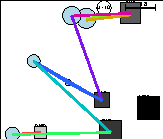
\includegraphics[width=.3\textwidth]{bilder/GreedyBesser-Greedy.pdf}
		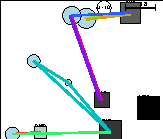
\includegraphics[width=.3\textwidth]{bilder/GreedyBesser-It.pdf}
		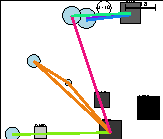
\includegraphics[width=.3\textwidth]{bilder/GreedyBesser-OPT.pdf}
		\caption{Die einzige Instanz, auf der die Greedy-Strategie die iterative schlägt \\ (Greedy-Lsg, iterative Lsg, optimale Lsg)}\label{fig:GreedyBesser}
	\end{figure}

\newpage

\section*{Ausblick}
	
Wir haben nun also gesehen wie Large Demand- und Merge-Phase des \CLR-Algorithmus so angepasst werden können, dass dieser auch für \CLRHFC-Instanzen zulässige Lösungen findet. Ferner hat die heuristische Betrachtung gezeigt, dass dabei zumindest in der euklidischen Ebene bereits meist eine akzeptable Approximationsgüte erreicht wird. Gleichzeitig zeigt aber \Cref{satz:schlechteApproximationsguete}, dass es - ebenfalls schon in der euklidischen Ebene - auch Instanzen gibt, auf denen die Approximation beliebig schlecht wird.
	
Eine naheliegender nächster Schritt auf der Suche nach einem guten Approximationsalgorithmus wäre nun auch die \UFL- und \MST-Phasen anzupassen, sodass die Fabrikkapazitäten bereits dort eine Rolle spielen. Zumindest für den \UFL-Teil sind hierzu auch passende Approximationsalgorithmen bekannt (z.B. \cite{Pal01facilitylocation}), allerdings zeigt etwa das in \cref{fig:bsp:schlechterMST} gezeigte Beispiel, dass dies allein vermutlich nicht ausreichen wird, da auch das Finden eines guten Spannbaums eine zentrale Rolle spielt.

Zudem ergibt sich durch das Einführen von Fabrikkapazitäten noch ein neues Problem im Zusammenspiel der \UFL- und \MST-Lösung (selbst wenn die Kapazitäten in diesen berücksichtigt werden): Da ein Kunde in den beiden Lösungen im Allgemeinen mit verschiedenen Fabriken verbunden sein darf, kann es passieren, dass Kunden sich in der Merge-Phase gegenseitig Fabriken \glqq wegnehmen\grqq. 

Denn: Nur weil ein Kunde beispielsweise in der \MST-Lösung mit einer nahen Fabrik verbunden ist (was dann später zur Abschätzung der tatsächlichen Anbindungskosten dienen soll), ist noch nicht sicher gestellt, dass diese Anbindung auch noch verfügbar ist, wenn dieser Kunde in der Merge-Phase tatsächlich an die Reihe kommt. Es kann vielmehr auch passieren, dass die entsprechende Fabrik zu diesem Zeitpunkt bereits durch andere Kunden voll ausgelastet ist. Es ist anzunehmen, dass derartige Effekte die Beschränkung der Kosten der letztendlich gefundenen Lösung im Allgemeinen deutlich erschweren und eventuell noch weitere Anpassungen der Merge-Phase nötig machen.

\newpage	

\newpage
\nocite{*}
\printbibliography		
			
\end{document}
